% -----------------------------------------------------------------
% Document class: Article
\documentclass[ a4paper, twoside, 11pt]{article}
\usepackage{../../../macros-general}
\usepackage{../../../macros-article}
% Number of the handout, quiz, exam, etc.
\newcommand{\numero}{02}
\setcounter{numero}{\numero}

% -----------------------------------------------------------------
\begin{document}
\allowdisplaybreaks

\begin{center}
\Large Mec\'anica Vectorial (MECG-1001): Lecci\'on \numero \\[2ex]
\small \textbf{Semestre:} 2017-2018 T\'ermino II \qquad
\textbf{Instructor:} Luis I. Reyes Castro \qquad
\textbf{Paralelo:} 08
\end{center}
\fullskip

% =============================================
\begin{problem}
En el ensamble mostrado en la siguiente figura la barra $AB$ tiene una velocidad angular constante de 4 rad/s en el sentido de las manecillas del reloj. 

\begin{figure}[htb]
\centering
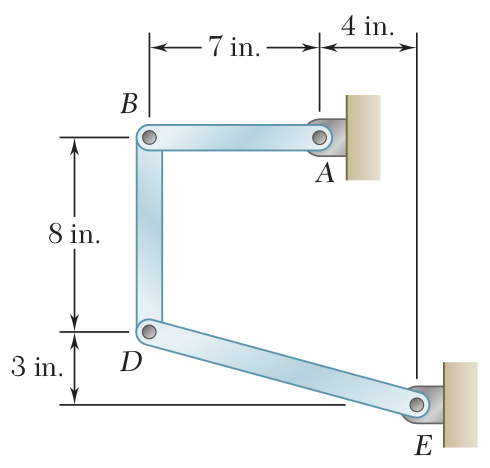
\includegraphics[width=0.38\textwidth]{problema-01.jpg}
\end{figure}

Complete las siguientes actividades: 
\begin{enumerate}[label=\textbf{\alph*)}]
\item \textbf{4 Puntos:} Encuentre las velocidades angulares de las barras $BD$ y $DE$. \\[1ex]
\emph{Soluci\'on:} Primero tomamos algunos datos: 
\begin{align*}
\vec{\hat{r}_{AB}} \; & = \; ( \, -1, \, 0 \, ) \\
\vec{r_{AB}} \; & = \; ( \, -7, \, 0 \, ) \; \text{in} \\
\vec{\hat{r}_{ED}} \; & = \; ( \, -0.9648, \, +0.2631 \, ) \\
\vec{r_{ED}} \; & = \; ( \, -11, \, +3 \, ) \; \text{in} \\
\vec{\hat{r}_{BD}} \; & = \; ( \, 0, \, -1 \, ) \\
\vec{r_{BD}} \; & = \; ( \, 0, \, -8 \, ) \; \text{in} \\
\vec{\omega_{AB}} \; & = \; -4 \; \uvec{k} \; \text{rad/s} \\
\vec{\alpha_{AB}} \; & = \; \vec{0} \; \text{rad/s\tsup{2}}
\end{align*}
Luego, reconocemos que las velocidades de $A$ y $B$ se relacionan con la velocidad angular de la barra $AB$ de la siguiente manera: 
\[
\vec{v_B}
\; = \; \vec{v_A} + \vec{\omega_{AB}} \cross \vec{r_{AB}}
\; = \; \colvec{0}{+28} \; \text{in/s}
\]
Similarmente, vemos que las velocidades de $D$ y $E$ se relacionan con la velocidad angular de la barra $DE$ de la siguiente manera: 
\[
\vec{v_D}
\; = \; \vec{v_E} + \vec{\omega_{DE}} \cross \vec{r_{ED}}
\; = \; \colvec{ -3 \, \omega_{DE}}{ -11 \, \omega_{DE}} \; \text{in/s}
\]
Finalmente, vemos que las velocidades de $B$ y $D$ se relacionan con la velocidad angular de la barra $BD$ de la siguiente manera: 
\begin{align*}
\vec{v_D} \;
& = \; \vec{v_B} + \vec{\omega_{BD}} \cross \vec{r_{BD}} \\
& = \; \colvec{0}{+28} + \colvec{ +8 \, \omega_{BD}}{0}
\; = \; \colvec{ +8 \, \omega_{BD}}{ +28} \; \text{in/s}
\end{align*}
Igualando las dos expresiones anteriores para la velocidad en $D$, tenemos: 
\begin{align*}
&
\colvec{ -3 \, \omega_{DE}}{ -11 \, \omega_{DE}}
\; = \; \colvec{ +8 \, \omega_{BD}}{ +28} \\
& \Longrightarrow \;
-11 \, \omega_{DE} \; = \; +28 \\
& \Longrightarrow \;
\vec{\omega_{DE}} \; = \; -2.546 \; \uvec{k} \; \text{rad/s} \\
& \Longrightarrow \;
\vec{\omega_{BD}} \; = \; +0.9546 \; \uvec{k} \; \text{rad/s}
\end{align*}

\item \textbf{4 Puntos:} Encuentre las aceleraciones angulares de las barras $BD$ y $DE$. \\[1ex]
\emph{Soluci\'on:} Primero, reconocemos que las aceleraciones de $A$ y $B$ se relacionan con la aceleraci\'on angular de la barra $AB$ de la siguiente manera: 
\begin{align*}
\vec{a_B} \;
& = \; \vec{a_A} + \vec{\alpha_{AB}} \cross \vec{r_{AB}} - \omega_{AB}^2 \, \vec{r_{AB}} \\
& = \; \vec{0} + \vec{0} -(-4)^2 \colvec{-7}{0} \; = \; \colvec{+112}{0} \; \text{in/s\tsup{2}}
\end{align*}
Similarmente, vemos que las aceleraciones de $D$ y $E$ se relacionan con la velocidad y aceleraci\'on angular de la barra $DE$ de la siguiente manera: 
\begin{align*}
\vec{a_D} \;
& = \; \vec{a_E} + \vec{\alpha_{DE}} \cross \vec{r_{ED}} - \omega_{DE}^2 \, \vec{r_{ED}} \\
& = \; \vec{0} + \colvec{ -3 \, \alpha_{DE}}{ -11 \, \alpha_{DE}} - (-2.546)^2 \, \colvec{-11}{+3} \\
& = \; 
\colvec{ +71.30 - 3 \, \alpha_{DE}}{ -19.47 - 11 \, \alpha_{DE}} \; \text{in/s\tsup{2}}
\end{align*}
Finalmente, vemos que las aceleraciones de $B$ y $D$ se relacionan con la velocidad y aceleraci\'on angular de la barra $BD$ de la siguiente manera: 
\begin{align*}
\vec{a_D} \;
& = \; \vec{a_B} + \vec{\alpha_{BD}} \cross \vec{r_{BD}} - \omega_{BD}^2 \, \vec{r_{BD}} \\
& = \; \colvec{+112}{0} + \colvec{ +8 \, \alpha_{BD}}{0} - (+0.9543)^2 \, \colvec{0}{-8} \\
& = \; 
\colvec{ +112 + 8 \, \alpha_{BD}}{+7.286} \; \text{ft/s\tsup{2}}
\end{align*}
Igualando las dos expresiones anteriores para la aceleraci\'on en $D$, tenemos: 
\begin{align*}
&
\colvec{ +71.30 - 3 \, \alpha_{DE}}{ -19.47 - 11 \, \alpha_{DE}} \; = \; \colvec{ +112 + 8 \, \alpha_{BD}}{+7.286} \\
& \Longrightarrow \;
-19.47 - 11 \, \alpha_{DE} \; = \; +7.286 \\
& \Longrightarrow \;
\vec{\alpha_{DE}} \; = \; -2.4324 \; \uvec{k} \; \text{rad/s\tsup{2}} \\
& \Longrightarrow \;
\vec{\alpha_{BD}} \; = \; -4.1754 \; \uvec{k} \; \text{rad/s\tsup{2}}
\end{align*}


\end{enumerate}

\end{problem}
\fullskip

% =============================================
\begin{problem}
\textbf{[6 Puntos]} Dos discos uniformes y dos cilindros est\'an ensamblados de la manera como se muestra en la siguiente figura. El disco $A$ pesa 20 lb y el disco $B$ pesa 12 lb. Si el sistema se suelta desde el reposo, encuentre las aceleraciones angulares de los discos y las aceleraciones translacionales de los cilindros. 

\begin{figure}[htb]
\centering
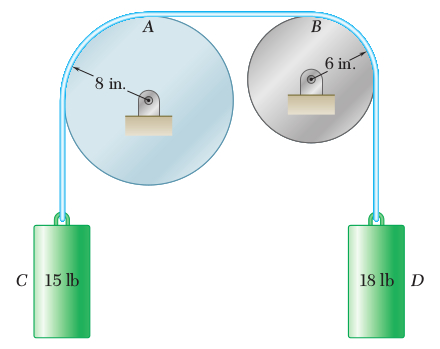
\includegraphics[width=0.50\textwidth]{problema-02.jpg}
\end{figure}

\end{problem}
\fullskip

% =============================================
\begin{problem}
\textbf{[4 Puntos]} La plataforma de 9 kg est\'a soportada, como se muestra en la siguiente figura, por dos discos uniformes que ruedan sin deslizarse en todas las superficies de contacto. La masa de cada disco es de 6 kg y el radio de 80 mm. Si se sabe que el sistema est\'a inicialmente en reposo, determine la velocidad de la plataforma despu\'es de que \'esta se haya desplazado 250 mm. 

\begin{figure}[htb]
\centering
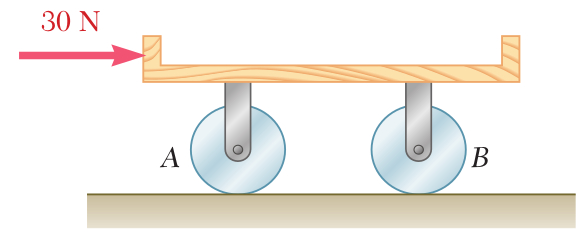
\includegraphics[width=0.5\textwidth]{problema-03.jpg}
\end{figure}

\end{problem}
\fullskip

% =============================================
\begin{problem}
Dos barras ligeras id\'enticas $AB$ y $BC$ se sueldan entre si para formar un mecanismo en forma de $L$, el cual se presiona contra un resorte en $D$ y se suelta desde la posici\'on indicada, tal como se muestra en la siguiente figura. Se sabe que el \'angulo m\'aximo de rotaci\'on del mecanismo en su movimiento subsecuente es de 90\deg en sentido contrario al de las manecillas del reloj. 

\begin{figure}[htb]
\centering
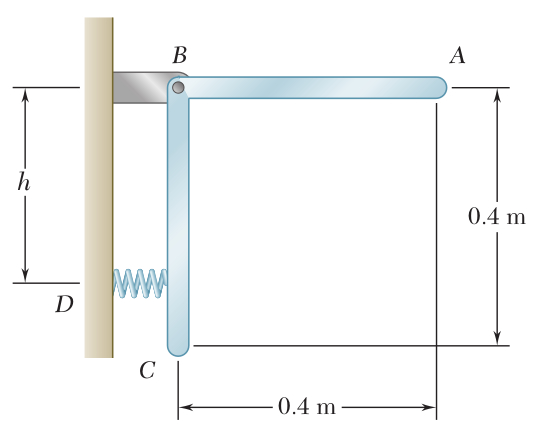
\includegraphics[width=0.4\textwidth]{problema-04.jpg}
\end{figure}

Complete las siguientes actividades: 
\begin{enumerate}[label=\textbf{\alph*)}]
\item \textbf{1 Punto:} Calcule la inercia del ensamble alrededor de $B$. 
\item \textbf{5 Puntos:} Determine la magnitud de la velocidad angular del mecanismo cuando pasa por la posici\'on en la que la barra $AB$ forma un \'angulo de 30\deg con la horizontal. 
\end{enumerate}

\end{problem}
\fullskip

\end{document}